
%% The following is a directive for TeXShop to indicate the main file
%!TEX root = ../MJThesis.tex
\acresetall
\resetlinenumber[1]
\chapter{Conclusions}
\label{ch:conclusions}
\begin{epigraph}
  \emph{``We must never let ourselves fall in thinking `ignorabimus' (`We shall never know'), but must have every confidence that the day will dawn when even those processes of life which are still a puzzle today will cease to be inaccessible to us natural scientists.''}\\ ---~Eduard~Buchner,~1907~Nobel~lecture 
\end{epigraph}
\section{Relevance and contribution to the field}\label{sec:relev-contr-field} 

\lettrine[lines=2]{T}{he} \textit{Caulobacter} field is dominated by research groups teasing apart the fine details of the \acl{caulobacter} lifecycle and the panoply of regulatory networks that control every aspect of bacterial biology. The \ac{S-layer}
 and the outer membrane often are neglected by the rest of the field. The focus
 on laboratory cultures, and not the bacteria in the environment, is one reason
 for this. A pure culture living in rich medium does not have as complex a
 relationship with its environment as a wild specimen competing in a hostile
 setting. It is the cell envelope that acts as the barrier between the world and
 the cell.  The cell envelope of \caulobacter{} was particularly suitable for inspection because it had a \acl{S-layer}, various \aclp{PS} including an \ac{OPS} of unknown structure, and apparently no porins. There is the added aspect that \caulobacter{}, and its \ac{S-layer}, are actively being pursued for biotechnology applications. This means that new findings can often be quickly be applied towards biological products. This work presented in chapters \ref{ch:crystal} \ref{ch:lps}, and \ref{ch:porin} present our efforts to improve the structure and composition knowledge of the \ac{S-layer}, \ac{LPS}, and outer membrane proteins in \caulobacter{}.
 
% The work in this dissertation also is focused on pure cultures in a laboratory setting, to its detriment. \Cref{ch:crystal} would have benefitted from information about how \acp{S-layer} increase fitness for wild \caulobacter{}.  \cref{ch:lps}  
\Cref{ch:crystal} detailed effort to solve the structure of RsaA. Protein crystallography is the only approach applicable to extend our current resolution of the \caulobacter{} \ac{S-layer} protein. \Ac{S-layer} proteins are notoriously resistant to crystallography. The work of Pavkov \etal{}\upcite[]{Pavkov20081226} and Baranova \etal{}\upcite[]{baranova2012sbsb} demonstrated that at least portions of \ac{S-layer} proteins are possible to crystallize as long as the ability for the proteins to form \acp{S-layer} is blocked. Our strategy to impede \ac{S-layer} formation was a truncation approach, removing the N-terminal 222 \ac{aa}, which mirrored the successful approach used to solve SbsC\upcite[.]{Pavkov20081226} Novel protein expression and purification techniques had to be developed to produce well-behaved protein suitable for crystallography. Once we started to grow crystals, RsaA was set to be the third bacterial \ac{S-layer} protein to be structurally solved, the second with the symmetry determining domain intact, the first from a Gram-negative, and the largest. But so far, finding a phasing solution has been the issue that is insurmountable. No phasing approach was successful, not the halide soaks that we had predicted would work, nor the lanthanide soaks that had worked for other groups\upcite[,]{baranova2012sbsb} nor any of a large range of  compounds tried. The C-terminal 804 \acp{aa} segment of RsaA has been crystallized, but the structure remains elusive. Solving this structure would provide the field with unique window into a self-assembling protein lattice from a commonly studied Gram-negative model organism. 

\ac{LPS} structures solutions are not as rare as \ac{S-layer} structures and yet
the complete structure of the \caulobacter{} \ac{LPS} had never been determined
when we started the work covered in \cref{ch:lps}. The \caulobacter{} lipid A
structure was solved by Smit \etal{} in 2008\upcite[,]{caulobacterlipida}
revealing a novel structure lacking phosphates and centered on a
di-diaminoglucose backbone. The structures of the \ac{OS} and \ac{OPS} were
identified for analysis because their fine structures had never been determined
and because they comprise the anchor for the \caulobacter{}
\ac{S-layer}\upcite[.]{walker94} An initial component analysis of the core
\ac{OS} was undergone in 1992\upcite[.]{ravenscroftlps} The \ac{OPS} had never
been studied directly but it was predicted that it was composed of
perosamine\upcite[.]{awramgenes} Through a very successful collaboration with
Dr. Evgeny Vinogradov the structures of the \caulobacter{} \ac{OS} and \ac{OPS}
are now determined. The core \ac{OS} has a three armed configuration (see
\cref{fig:lpscore} on \cpageref{fig:lpscore}). The final determined components
of the core \ac{OS} are different than were first
reported\upcite[,]{ravenscroftlps} especially in the finding that there is no
phosphate in the core \ac{OS}. The first arm is a disaccharide of glucuronic
acid and galactose. The two negative charges in the galacturonic acids in the
lipid A, the one in the central Kdo, and the one in the glucuronic acid are the
only charges present in the \caulobacter{} \ac{LPS}. The second arm is a
trisaccharide of DD-heptose, mannose, and DL-heptose. The third arm is a single
DL-heptose, linked to the C-7 position of the Kdo moiety. This triple
substitution on the Kdo appears to be unique in the literature. There are
examples of sugar substitutions at all of the same positions (C-4, C-5, and C-7)
in Kdo but none for all three at once. The \ac{OPS} has a repeating
heptasaccharide structure (see \cref{fig:lpsops} on \cpageref{fig:lpsops}).
Seven sugar \ac{OPS} subunits are amongst the largest sizes that subunits are
known to exist in. For example, there is just one known example of a seven sugar
\ac{OPS} in \acl{ecoli}, and none larger\upcite[.]{stenutz2006structures} The
\caulobacter{} \ac{OPS} terminates in one or the other of two end groups (see
\cref{fig:lpsends} on \cpageref{fig:lpsends}).  A complete structural view of
the \caulobacter \ac{LPS} is shown in \cref{fig:fulllps}. Both the \ac{OPS} and end groups contain an abundance of hydrophobic sugars, \ie N-acetylperosamine, rhamnose, methylglucose, and dimethyl-N-acetylperosamine. There may be a role for this hydrophobicity to play in supporting an \ac{S-layer}. The \ac{OPS} composition of \textit{Aeromonas hydrophila} AH-1\upcite[,]{merino2015molecular} another alphaproteobacterium with an \ac{S-layer}, supports this hypothesis; one in two monosaccharides in its \ac{OPS} is the deoxysugar acetylrhamnose. In the process of studying the \caulobacter{} \ac{LPS} we discovered a previously unknown rhamnose based polysaccharide (see \cref{fig:lpsrhamnan} on \cpageref{fig:lpsrhamnan}). Just the presence of the polysaccharide alone is of interest especially in light of recent investigations into the \acp{EPS} from \caulobacter{} by the Viollier lab at the University of Geneva\upcite[.]{ardissone2014cell}  

\begin{figure}[p]
  	\begin{center}
   		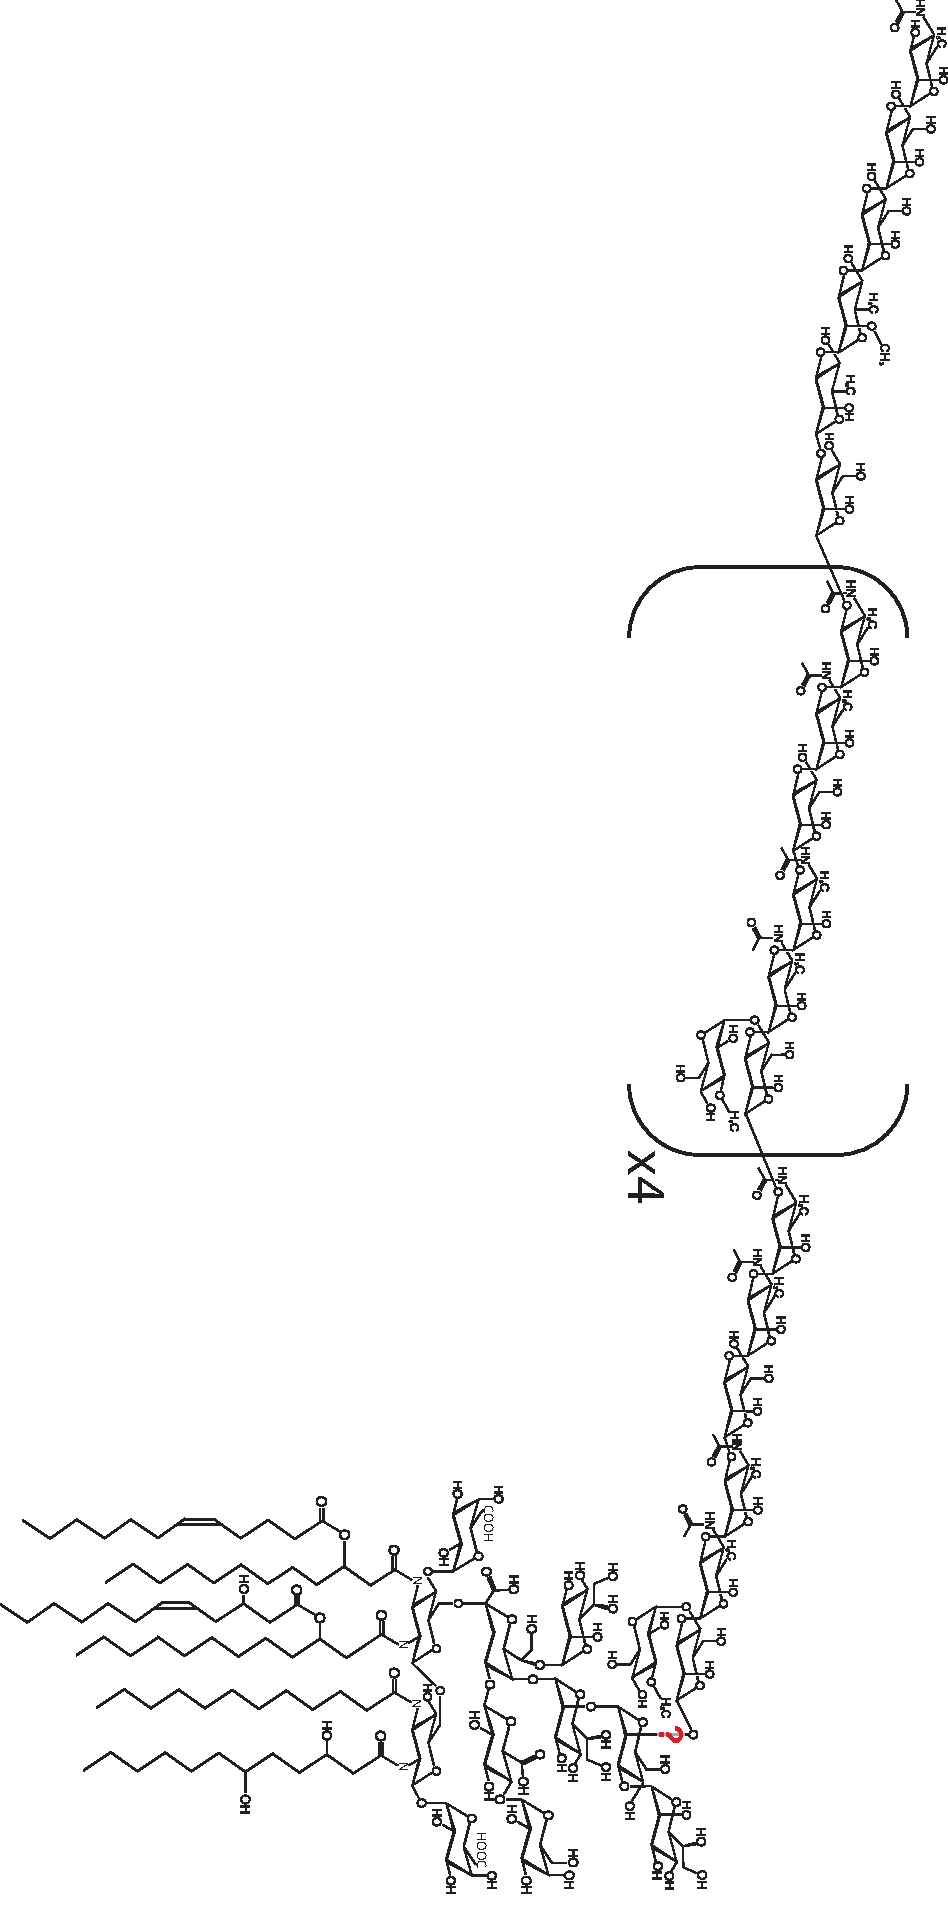
\includegraphics[height=0.89\textheight]{conclusion_chapter/img/fulllps.pdf}
   	\end{center}
   	\caption[The complete structure of the \caulobacter \ac{LPS}]{The fully
      assembled structure of the \caulobacter \ac{LPS}. Included is the lipid A,
    the core oligosaccharide, five repeats of the \ac{OPS}, and the longer of
    the two possible end groups. The red question mark denotes the one currently
  undetermined linkage, the bond between the \ac{OPS} and the core.}
\label{fig:fulllps}
\end{figure}

\Cref{ch:porin} reports our characterization of OmpW, a porin in the outer membrane of \caulobacter{}. Previous to this work, no porin had been reported in \caulobacter{}. The wisdom on the subject was that \caulobacter{} primarily, if not solely, used active transport systems to take up nutrients from the environment\upcite[.]{lohmiller2008tonb} We found that OmpW acts as a passive protein channel in the outer membrane (see \cref{fig:porin-20ksinglechannel}). This is particularly interesting because the homologous proteins in \ecoli{} and \acl{pseudomonas} do not have any pore forming activity\upcite[]{hong2006outer, touw2010crystal} and no clear function at all.  The activity we observed is possibly due to a wider pore and specifically a lack of a plug seen in the other bacteria.  

\section{Future directions}\label{sec:future-directions}

Each aspect of this work, the protein crystallography, the \ac{LPS} analyses, and characterization of OmpW, opened more questions than they answered. One goal of this work has always been to use all the gains made with basic science to improve the \caulobacter{} \ac{S-layer} display technology in the Smit lab. The rewards in biotechnology pursuits are not yet obvious, though a complete knowledge of the \ac{LPS} will undoubtedly guide efforts to assemble \acp{S-layer} on abiotic surfaces.

The RsaA crystallography is the obvious loose end in this dissertation. We do not have the structure of RsaA solved to atomic resolution; this means the phase problem must be solved. It is possible that a particular compound exists or a certain soaking protocol exists that will provide us our solution. It is possible that the next RsaA \del 0--222 crystal grown will have the best diffraction yet and will give a nice clean signal. It is possible that we continue on our path and we will figure this out. We will continue trying the same approaches but doing only that cannot be the only way forward. The halides, specifically iodine, were the best candidates to consider at the beginning and we indeed got some very enticing early data from them. It seemed that small optimizations might be satisfactory to complete the project. We got drawn in by these successes and it delayed us trying new strategies.

Our troubles with phasing are at least in part due to a dearth of useful
residues in the protein to couple with heavy atoms. For instance, there are too few methionines for seleomethionine incorporation (if that was possible in \caulobacter{}) and there are no cysteines which limits the use of many heavy metals\upcite[.]{islam1998had} We can modify RsaA to contain any residues we want, at least at selected positions within RsaA; this is the strategy we have already begun with our GSCC cassette insert (see \cref{sec:stra-plasm-constr}). Cysteine-rich and methionine-rich inserts at positions known to tolerate heterologous insertions (\eg \ac{aa} 644, 690, 723, 784, 805, and 944) are obvious approaches to be tried. As of this writing, cloning has begun to insert various peptides into RsaA for the purposes of improving our phasing. We do have to consider the possibility that the insert-strategy is inherently flawed. We saw that our GSCC inserted RsaA did not crystallize well. The cause for that is not clear and it is possible that there is a structural instability introduced by exogenous peptides. Less common methods, like molecular replacement from a low resolution cryo-electron microscopy structure\upcite[,]{jore2011structural} are also possibilities that should be considered. 

Once we have figured out our difficulties with the RsaA structural analysis, we can start to assess the
current peptide display strategies in the context of a protein  structure.
Rational design choices can then be used to improve the display products. Currently display peptides are inserted into \textit{rsaA} at sites that were first found by trial-and-error and evaluated by many years of use\upcite[.]{bingle1997linker} Despite their consistent efficacy, we do not know how these display sites fit into the structure of RsaA. Locating sites on RsaA that are less buried in the protein may improve peptide accessibility to the environment. Choosing display sites with increased flexibility may allow for more complex tertiary structures for the display peptides to adopt. 

Designing the insert peptides with respect to how they fit into the larger
three-dimensional structure of the \ac{S-layer} may open up new directions of
innovation. For example, we can currently co-display two-separately engineered
versions of RsaA on the surface of a single \caulobacter cell. But with more
fine-detail information about RsaA's structure, we could imagine displaying two
types of RsaA each containing  a specifically arranged half of a functional
dimer that assembles in the \ac{S-layer}. Another example that would be of
immediate interest to our laboratory would be to improve the targeting of HIV.
\caulobacter and RsaA constructs have been created in our laboratory that
inhibit HIV entry into T-cells\upcite[.]{nomellini2010development, hivmicrobicide2} The three copies of RsaA in the center of three-fold symmetry in the \ac{S-layer} (see \cref{fig:intro-micrograph}) could each display a GP120-binding peptide, rationally spaced to match the trimer structure of GP120.

The \ac{LPS} of \caulobacter{} is presented in \cref{ch:lps} but the study of
\textit{Caulobacter}'s outer membrane polysaccharides is not complete.
Specifically for the \ac{OPS}, there is one glycosidic bond that was not
abundantly clear in our data. The linkage between the \ac{OPS} and the core
oligosaccharide is still unknown (see \cref{fig:fulllps}). This  single bond is particularly difficult to determine because it is present in \ac{NMR} spectra alongside the highly amplified data coming from the repeating \ac{OPS} structure. A project is underway to double our efforts to identify that one missing bond by \ac{NMR}. That bond could possibly  be determined through genetic knockouts. There are six sugars in the core oligosaccharide that could be the base of the \ac{OPS}, but only three sugars if we assume it is on the C-5 branch from the Kdo (as is common in LPS). If we knockout the glycosyltransferase responsible for adding the base sugar that supports the \ac{OPS}, then we would see a loss of smooth-\ac{LPS}. But that points out another gap in our understanding: the genetics of the \caulobacter{} \ac{LPS} are still an open question. The work of Awram \etal{} (2001) did the first survey of \ac{OPS} biosynthetic genes\upcite[,]{awramgenes} but now we could go back and start identifying these genes' functions based on changes in polysaccharide structure. Only one true \ac{LPS} synthesis protein from \caulobacter{} has been characterized, LpxI\upcite[]{lpxi} (this study misidentified the \caulobacter lipid A precursors to be glucosamines instead of diaminoglucoses); there are many more to be studied. 

Even before that last bond is determined, progress can continue to use the \ac{LPS} to improve the \textit{Caulobacter} peptide-display technology and move \acp{S-layer} onto abiotic surfaces. \Ac{NMR} analysis demonstrated that we can liberate free-\ac{OPS} by mild-acid hydrolysis and that there are carboxyl groups present on the Kdo that can be chemically linked to an amine\upcite[.]{jauho2000new} We should redouble our efforts to chemically produce \ac{OPS} functionalized surfaces, regardless of our previous negative results.  Additionally, working with the Cullis Lab in the Department of Biochemistry and Molecular Biology at UBC, lipid nanoparticles\upcite[]{leung2015microfluidic} have been created that are in part  composed of \caulobacter \ac{LPS}. The ultimate goal is to produce nanoparticles that display therapeutic targeting molecules. The work is preliminary but they have already been produced in various sizes and have been loaded with siRNA or fluorescent dyes. Efforts to demonstrate successful formation of \acp{S-layer} of recombinant RsaA onto the nanoparticles are underway. Thus nanoparticles  may be potent platforms to support an \ac{S-layer} peptide-display technology.

A further area of future study is the new rhamnan polysaccharide. I am particularly interested in what role this rhamnan polysaccharide plays in the cells' lifestyle. There are questions to be asked related to how it affects sedimentation rates, surface adhesion,  and phage resistance. Discovering a new polysaccharide, rhamnan polysaccharide, like our discovery that OmpW acts as a outer membrane channel, begs the question of what else lies in the outer membrane and cell envelope waiting to be discovered next?
